\documentclass[addpoints,12pt,answers]{exam}
\usepackage[top=1in, bottom=1in, left=.45in, right=.45in]{geometry}
\usepackage{amsmath,amscd,amssymb,amsthm,fontsize}
\usepackage{setspace,graphicx, enumerate}
\usepackage{multirow}
\usepackage{pgf,pgfplots,pgfkeys}
\usepackage{tikz, comment, twoopt}
\usepackage{multicol}

\usetikzlibrary{arrows}
\setlength{\unitlength}{1in}

\newcommand{\NN}{\mathbb{N}}
\newcommand{\RR}{\mathbb{R}}
\newcommand{\II}{\mathbb{I}}
\newcommand{\QQ}{\mathbb{Q}}
\newcommand{\ZZ}{\mathbb{Z}}

%%%%%%%%%%%%%%%%%%%%%%%
%Font & Size Adjustments
%%%%%%%%%%%%%%%%%%%%%%%
\usepackage[T1]{fontenc}
\usepackage{arev}
\renewcommand\bfdefault{bx}
\renewcommand{\familydefault}{\sfdefault}

\changefontsize{14pt}

\usepackage[most]{tcolorbox}

%Also need to change Standard Response Questions box and Congratulations box!

%%%%%%%%%%%%%%%%%%%%%%%
%Definitions of things
%%%%%%%%%%%%%%%%%%%%%%%
\newcommand{\ds}{\displaystyle}

\newenvironment{ansb}[2]
			{\begin{flushright}
			\begin{tikzpicture}
			\draw[fill=black] (.1,-.1) rectangle ({#1+.1},{#2-.1});
			\draw[fill=white] (0,0) rectangle (#1,#2);
			\draw (.8,{#2+.2}) node {\textbf{Answer:}};}
			{\end{tikzpicture}\end{flushright}}
\newenvironment{soln}
      {\let\oldqedsymbol=\qedsymbol
      \renewcommand{\qedsymbol}{$ $}
      \begin{proof}[\bfseries\upshape \color{blue}Solution]\color{blue}}
      {\end{proof}
      \renewcommand{\qedsymbol}{\oldqedsymbol}}


%===========================================================
%%%%%%%%%%%%%%%%%%%%%%%%%%%%%%%%%%%%%%%%%%%%%%%%%%%%%%%%%%%%
%Change for each exam
%%%%%%%%%%%%%%%%%%%%%%%%%%%%%%%%%%%%%%%%%%%%%%%%%%%%%%%%%%%%
\newcommand{\course}{MATH 0482 (Revised FA24)}
%\newcommand{\edate}{December 4th, 2023}
\newcommand{\edate}{Initials: \hspace{.35in}}
\newcommand{\exam}{Midterm Exam}
\newcommand{\exammin}{\textbf{2 hours}}
%%%%%%%%%%%%%%%%%%%%%%%%%%%%%%%%%%%%%%%%%%%%%%%%%%%%%%%%%%%%
%CHANGE FOR SOLUTIONS
%%%%%%%%%%%%%%%%%%%%%%%%%%%%%%%%%%%%%%%%%%%%%%%%%%%%%%%%%%%%
\noprintanswers
%\printanswers
%===========================================================

%%%%%%%%%%%%%%%%%%%%%%%
%Header and footer info - No need to change
%%%%%%%%%%%%%%%%%%%%%%%
\pagestyle{headandfoot}
\firstpageheadrule
\runningheadrule
\firstpageheader{\course}{
\ifprintanswers
Solutions to
\fi
\exam}{\edate}
\runningheader{\course}{
\ifprintanswers
Solutions to
\fi
\exam}{\edate}
\firstpagefooter{$\star$}{}{Page \thepage\ of \numpages}
\runningfooter{}{}{Page \thepage\ of \numpages}


%%%%%%%%%%%%%%%%%%%%%%%
%Extra code that the exam environment will except
%%%%%%%%%%%%%%%%%%%%%%%
%\ifprintanswers
%Stuff to appear only when answers are being printed.
%\else
%Stuff to appear only when answers are not being printed.
%\fi

%\numquestions
%\numparts
%\numsubparts
%\numsubsubparts
%\numpoints
%\numbonuspoints


%%%%%%%%%%%%%%%%%%%%%%%
%Changes color of fill in the blank answers.
%%%%%%%%%%%%%%%%%%%%%%%
\ifprintanswers 
	\newcommand{\sd}[1]{\textcolor{blue}{#1}}
\else 
	\newcommand{\sd}[1]{\textcolor{white}{#1}}
\fi
	\newcommand{\und}[2][0in]{\underline{\sd{#2}}\underline{\phantom{#2} \hspace{#1}}}

%%%%%%%%%%%%%%%%%%%%%%%
%Exam settings (grade table, points, solutions)
%%%%%%%%%%%%%%%%%%%%%%%
\cellwidth{2em}
\gradetablestretch{1.5}
%\bracketedpoints
%\boxedpoints
\shadedsolutions
\definecolor{SolutionColor}{rgb}{0.8,0.9,1}

\CorrectChoiceEmphasis{\Large\color{blue}}

%%%%%%%%%%%%%%%%%%%%%%%
%Exam cover page - no need to change, updates automatically
%%%%%%%%%%%%%%%%%%%%%%%
\begin{document}
\phantom{.}
\vspace{.2cm}

\noindent \textbf{Name}: 
\rule{.5\textwidth}{.2mm} \hspace{1cm} \textbf{ID:}
\hrulefill \\ 

%\vspace{.5cm}

%\noindent \textbf{Section}: \rule{.2\textwidth}{.2mm} \hspace{1cm}
%\textbf{Recitation Instructor}: \hrulefill

\vspace{.2cm}
\fontsize{12}{12}\selectfont{
\textbf{INSTRUCTIONS}\\[8pt]
\phantom{.}\hspace{.7cm}
\begin{minipage}{6.3in}
	\begin{itemize}
		%\setlength{\itemindent}{1cm}
		\item Fill in your name, etc. on this first page. Write your initials on the top right of each page.
		\item Without fully opening the exam, check that you have pages 1 through \totalnumpages.
		\item {\bf Show all your work} on the standard response questions. Write your answers clearly!  Include enough steps for the grader to be able to follow your work. Include words to clarify your reasoning.
		\item Do first all of the problems you know how to do immediately. Do not spend too much time on any particular problem. Return to difficult problems later.
		\item If you have any questions please raise your hand and the instructor will come to you.
		\item You will be given exactly \exammin \ for this exam.
		%\item You may use a \textbf{SINGLE PAGE} (8.5'' by 11'') of \textbf{HANDWRITTEN} notes (front and back).
		\item A SCIENTIFIC calculator may be used on the exam. \textbf{No graphing calculators are permitted on this exam}.
	\end{itemize}
\end{minipage}

\vspace{.2cm}

\textbf{ACADEMIC HONESTY}\\[8pt]
\phantom{.}\hspace{.7cm}
\begin{minipage}{6.3in}
	\begin{itemize}
		
		\item Do not open the exam booklet until you are instructed to do so.
		\item Do not seek or obtain any kind of help from anyone to answer questions on this exam. If you have questions, consult only the instructor.
		\item Books, notes, phones, or any other electronic devices are \textbf{not} allowed on the exam. Students should store them in their backpacks.
		%\item No scratch paper is permitted. If you need more room use the back of a page. 
		\item Anyone who violates these instructions will have committed an act of academic dishonesty.
		Penalties for academic dishonesty can be very severe. All cases of academic dishonesty will be reported immediately to the Mathematics Department Chair and then the Dean of Math and Science.
	\end{itemize}
\end{minipage}

\vspace{1cm}

\noindent I have read and understand the\\ above instructions and statements\\ regarding academic honesty:  \, \, \hrulefill\\
\ {\color{white} .} \hspace{11 cm} \textbf{{\footnotesize SIGNATURE}}}


\vfill

\newpage
\phantom{.}
\vfill
\begin{center}
   \textit{This page is intentionally left blank}.
\end{center}
\vfill

\newpage

%%%%%%%%%%%%%%%%%%%%%%%%%%%%%%%%%%%%%%%%%%%
% STANDARD RESPONSE BOX WITH INSTRUCTIONS %
%%%%%%%%%%%%%%%%%%%%%%%%%%%%%%%%%%%%%%%%%%%

\begin{tcolorbox}[colback=gray!15,colframe=black]
		{\textbf{Standard Response Questions}. Show all work to receive credit. Please \fbox{\textbf{BOX}} your final answer. }
\end{tcolorbox}



\vspace{-.5cm}

%%%%%%%%%%%%%%%%%%%%%%%%%%%%%%%%%%%%%%%%%%%%%%
% START WRITING STANDARD RESPONSE QUESTIONS HERE
%%%%%%%%%%%%%%%%%%%%%%%%%%%%%%%%%%%%%%%%%%%%%%




\begin{questions}

\question[5] Simplify: $8 - 3( 14 - |4 - 5^2| )$
\begin{solution}
$8 - 3( 14 - |4 - 5^2| )$ 

 $= 8 - 3( 14 - |4 - 25| )$ 

 $= 8 - 3( 14 - |-21| )$ 

 $= 8 - 3( 14 - 21 )$ 

 $= 8 - 3( -7 )$ 

 $= 8 - ( -21 )$ 

 $= \boxed{ 29 }$
\end{solution}
\vspace{\stretch{1}}\answerline


\question[5] Simplify the radical expression completely: 

 $7 \sqrt[5]{ -96 }$
\begin{solution}
$7 \sqrt[5]{ -96 }$ 

 $= 7 \cdot \sqrt[5]{ -32 \cdot 3 }$ 

 $= 7 \cdot (-2) \sqrt[5]{ 3 }$ 

 $= \boxed{ -14 \sqrt[5]{ 3 } }$
\end{solution}
\vspace{\stretch{1}}\answerline


\question[5] Simplify: $\displaystyle \left( \frac{ -3 a^{0} b^{-4} c^{-1} }{ a^{4} b^{-2} c^{-3} } \right)^{ -2 }$
\begin{solution}
$\displaystyle \left( \frac{ -3 a^{0} b^{-4} c^{-1} }{ a^{4} b^{-2} c^{-3} } \right)^{ -2 }$ 

 $= \left( -3 a^{-4} b^{-2} c^{2} \right)^{-2}$ 

 $= (-3)^{-2} a^{8} b^{4} c^{-4}$ 

 $= \boxed{ \frac{a^{8}b^{4}}{9c^{4}} }$
\end{solution}
\vspace{\stretch{1}}\answerline

\newpage

\question[5] Simplify: $(2 \, x^{2} - 7 \, x + 5) - (3 \, x^{2} + 5 \, x - 4)$
\begin{solution}
$(2 \, x^{2} - 7 \, x + 5) - (3 \, x^{2} + 5 \, x - 4)$ 

 $= 2x^2-7x+5-3x^2-5x+4$ 

 $= 2x^2-3x^2-7x-5x+5+4$ 

 $= \boxed{ -x^{2} - 12 \, x + 9 }$
\end{solution}
\vspace{\stretch{1}}\answerline


\question[5] Simplify: $(2x - 2y)(4x^2 + 4xy + 4y^2)$
\begin{solution}
$(2x - 2y)(4x^2 + 4xy + 4y^2)$ 

 $= 2x(4x^2 + 4xy + 4y^2) - 2y(4x^2 + 4xy + 4y^2)$ 

 $= 8x^3 + 8x^2y + 8xy^2 - 8x^2y - 8xy^2 - 8y^3$ 

 $= \boxed{ 8x^3 - 8y^3 }$
\end{solution}
\vspace{\stretch{2}}\answerline


\question[5] Simplify: $\displaystyle \frac{ -2 \, x^{4} - 5 \, x^{3} - 6 \, x^{2} + 8 \, x + 4 }{ 2 \, x + 1 }$
\begin{solution}
$\begin{array}{r} -x^{3} - 2 \, x^{2} - 2 \, x + 5 \\ 2 \, x + 1 \overline{ ) -2 \, x^{4} - 5 \, x^{3} - 6 \, x^{2} + 8 \, x + 4 } \\ \underline{ -( -2 \, x^{4} - x^{3} ) } \\\\ -4 \, x^{3} - 6 \, x^{2} + 8 \, x + 4 \\ \underline{ -( -4 \, x^{3} - 2 \, x^{2} ) } \\\\ -4 \, x^{2} + 8 \, x + 4 \\ \underline{ -( -4 \, x^{2} - 2 \, x ) } \\\\ 10 \, x + 4 \\ \underline{ -( 10 \, x + 5 ) } \\\\ -1 \end{array}$ 

 $= \boxed{ -x^{3} - 2 \, x^{2} - 2 \, x + 5 - \frac{1}{2 \, x + 1} }$
\end{solution}
\vspace{\stretch{2}}\answerline

\newpage

\question[5] Solve: $14 - 3(5x - 9) = 2(5x + 8)$
\begin{solution}
$14 - 3(5x - 9) = 2(5x + 8)$ 

 $14 - 15x + 27 = 10x + 16$ 

 $41 - 15x = 10x + 16$ 

 $41 = 25x + 16$ 

 $25 = 25x$ 

 $\boxed{ x = 1 }$
\end{solution}
\vspace{\stretch{1}}\answerline


\question[5] Solve: $\displaystyle \frac{1}{2}x + \frac{1}{3} = -4$
\begin{solution}
$\displaystyle \frac{1}{2}x + \frac{1}{3} = -4$ 

 $6 \left( \frac{1}{2}x + \frac{1}{3} = -4 \right)$ 

 $3x + 2 = -24$ 

 $3x = -26$ 

 $x = \frac{-26}{3}$ 

 $\boxed{ x = -\frac{26}{3} }$
\end{solution}
\vspace{\stretch{1}}\answerline


\question[5] Solve for $y$: $mx + ny = p$
\begin{solution}
$mx + ny = p$ 

 $ny = p - mx$ 

 $\boxed{ y = \frac{p - mx}{n} }$
\end{solution}
\vspace{\stretch{1}}\answerline

\newpage

\question[5] A cargo van costs \$$57.00$ per day plus \$$0.30$ per mile driven. If Bob has \$$120.90$ for a one-day rental, how many miles can they drive?
\begin{solution}
$120.90 - 57.00 = 63.90$ 

 $\frac{63.90}{0.30} = 213$ 

 $\boxed{ 213 \text{ miles} }$
\end{solution}
\vspace{\stretch{1}}\answerline


\question[5] Graph and identify the slope and $y$-intercept: \\

$f(x) = \displaystyle{ \frac{7}{8} }x + 7$

\begin{multicols}{2}
{\renewcommand{\arraystretch}{2.5}%
\begin{tabular}{|c|p{1.5in}|}\hline
    slope &  \\ \hline
    $y$-int &  \\ \hline
    $x$-int & \\ \hline
\end{tabular}}

\vspace{\stretch{1}}

\columnbreak
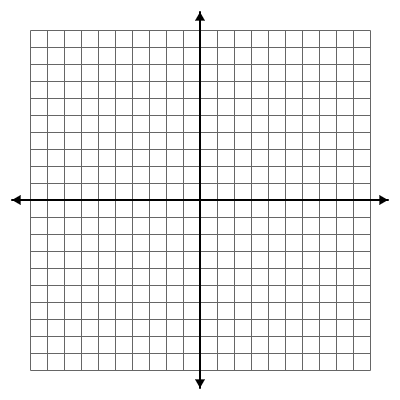
\includegraphics[width=3.5in]{blankgraph.PNG}

\end{multicols}

\begin{solution}
\(\text{Slope: } m = \frac{7}{8}\) 

 \(\text{y-intercept: } (0, 7)\) 

 \(\text{x-intercept: } (-8, 0)\) 

 \begin{tikzpicture}[scale=0.4] \draw[help lines, color=gray!50] (-10,-10) grid (10,10); \draw[<->, thick] (-10.5,0)--(10.5,0) node[right]{$x$}; \draw[<->, thick] (0,-10.5)--(0,10.5) node[above]{$y$}; \begin{scope} \clip (-10,-10) rectangle (10,10); \draw[<->, ultra thick, blue, domain=-11:11, samples=2] plot (\x, {0.875*\x + 7.0}); \end{scope} \fill[red] (-8,0) circle (0.3); \fill[red] (0,7) circle (0.3); \end{tikzpicture}
\end{solution}

\newpage

\question[5] Given $g(x) = x^2 - 2x + 6$, find each of the following.
\begin{parts}
  \part $g(-1)$
  \begin{solution}\(g(-1) = (-1)^2 - 2(-1) + 6\) 

 \(= 1 + 2 + 6\) 

 \(= \boxed{ 9 }\)\end{solution}
  \vspace{\stretch{1}}\answerline
  \part $g(0)$
  \begin{solution}\(g(0) = (0)^2 - 2(0) + 6\) 

 \(= \boxed{ 6 }\)\end{solution}
  \vspace{\stretch{1}}\answerline
  \part $g(x+h)$
  \begin{solution}\(g(x+h) = (x+h)^2 - 2(x+h) + 6\) 

 \(= \boxed{ x^2 + 2xh + h^2 - 2x - 2h + 6 }\)\end{solution}
  \vspace{\stretch{1}}\answerline
\end{parts}

\newpage
\uplevel{\textbf{For Problems \ref{func-1} and \ref{func-2}, identify the domain and range and determine whether or not the graph represents a function. If it is not a function, explain why.}}

\question[5]\label{func-1} \,

\begin{multicols}{2}

Function: \begin{oneparcheckboxes} \choice Yes \choice No \end{oneparcheckboxes}\\
\vspace{.25in} \\
\vspace{.25in}Explain: \hrulefill \\
\vspace{.25in}\hrulefill

{\renewcommand{\arraystretch}{2}%
\begin{tabular}{|c|p{1.5in}|}\hline
    Domain &  \\ \hline
    Range & \\ \hline
\end{tabular}}

\vspace{\stretch{1}}

\columnbreak
\centering
\begin{tikzpicture}[scale=0.35] \draw[step=1cm, gray!40, very thin] (-10,-10) grid (10,10); \draw[thick, <->] (-10.5,0) -- (10.5,0) node[right] {$x$}; \draw[thick, <->] (0,-10.5) -- (0,10.5) node[above] {$y$}; \foreach \x in {-10,-8,...,10} \draw (\x, 0.1) -- (\x, -0.1) node[below] {\tiny $\x$}; \foreach \y in {-10,-8,...,10} \draw (0.1, \y) -- (-0.1, \y) node[left] {\tiny $\y$}; \draw[ultra thick, blue, <->, domain=-3.0:5.0, samples=100] plot (\x, {-0.500000000000000*(\x - 1)^2 + -2}); \end{tikzpicture}

\end{multicols}

\begin{solution}
\begin{itemize}
\item
Domain: \((-\infty, \infty)\)

\item
Range: \((-\infty, -2]\)

\item
Function

\end{itemize}
\end{solution}
\vspace{\stretch{1}}


\question[5]\label{func-2} \,

\begin{multicols}{2}

Function: \begin{oneparcheckboxes} \choice Yes \choice No \end{oneparcheckboxes}\\
\vspace{.25in} \\
\vspace{.25in}Explain: \hrulefill \\
\vspace{.25in}\hrulefill

{\renewcommand{\arraystretch}{2}%
\begin{tabular}{|c|p{1.5in}|}\hline
    Domain &  \\ \hline
    Range & \\ \hline
\end{tabular}}

\vspace{\stretch{1}}

\columnbreak
\centering
\begin{tikzpicture}[scale=0.35] \draw[step=1cm, gray!40, very thin] (-10,-10) grid (10,10); \draw[thick, <->] (-10.5,0) -- (10.5,0) node[right] {$x$}; \draw[thick, <->] (0,-10.5) -- (0,10.5) node[above] {$y$}; \foreach \x in {-10,-8,...,10} \draw (\x, 0.1) -- (\x, -0.1) node[below] {\tiny $\x$}; \foreach \y in {-10,-8,...,10} \draw (0.1, \y) -- (-0.1, \y) node[left] {\tiny $\y$}; \draw[ultra thick, blue, <->, domain=-0.7416573867739413:6.741657386773941, samples=100] plot ({-0.500000000000000*(\x - 3)^2 + -3}, \x); \end{tikzpicture}

\end{multicols}

\begin{solution}
\begin{itemize}
\item
Domain: \((-\infty, -3]\)

\item
Range: \((-\infty, \infty)\)

\item
Not a function

\end{itemize}
\end{solution}

\newpage

\question[5] Given the graph of the function $f$, find each of the following.
\vspace{2em}
\begin{multicols}{2}
\centering
\begin{tikzpicture}[scale=0.35] \draw[step=1cm, gray!40, very thin] (-10,-10) grid (10,10); \draw[thick, <->] (-10.5,0) -- (10.5,0) node[right] {$x$}; \draw[thick, <->] (0,-10.5) -- (0,10.5) node[above] {$y$}; \foreach \x in {-10,-8,...,10} \draw (\x, 0.1) -- (\x, -0.1) node[below] {\tiny $\x$}; \foreach \y in {-10,-8,...,10} \draw (0.1, \y) -- (-0.1, \y) node[left] {\tiny $\y$}; \draw[ultra thick, blue, <->, domain=-5.3166247903554:1.3166247903553998, samples=100] plot (\x, {1*(\x - -2)^2 + -1}); \end{tikzpicture}

\columnbreak

\begin{parts}
  \part $f(0)$ = \fillin\vspace{2em}\\
  \part $f(-1)$ = \fillin\vspace{2em}\\
  \part $f(-3)$ = \fillin\vspace{2em}\\
  \part Find $x$ where $f(x) = -1$ \\[2em] $x=$ \fillin\vspace{2em}\\
\end{parts}
\end{multicols}

\begin{solution}
\begin{itemize}
\item
(a) \(3\)

\item
(b) \(0\)

\item
(c) \(0\)

\item
(d) \(x = -2\)

\end{itemize}
\end{solution}


\question[5] Find the equation of the line parallel to $6x - 2y = -2$ and passing through $(-5, -6)$.
\begin{solution}
Slope:

 $6x - 2y = -2$ 

 $-2y = -6x + -2$ 

 $y = 3x + 1$ 

 $m = 3$ 

Y-intercept:

 $y = mx + b$ 

 $-6 = 3(-5) + b$ 

 $-6 = -15 + b$ 

 $b = 9$ 

 $\boxed{ y = 3x + 9 }$
\end{solution}
\vspace{\stretch{1}}\answerline

\newpage

\question[5] A particular search engine assigns a ranking to a webpage based on the number of links that direct users to the webpage. The ranking of a webpage is given by the function below, where $n$ represents the number of links that direct users to it. How many links will be needed to obtain a page ranking of 9? 

 $R(n) = \frac{1}{23}n + 1$
\begin{solution}
$9 = \frac{1}{23}n + 1$ 

 $8 = \frac{1}{23}n$ 

 $184 = n$ 

 $\boxed{ 184 \text{ links} }$
\end{solution}
\vspace{\stretch{1}}\answerline


\question[5] Solve the system of equations. 

 $\begin{cases} x - y = -6 \\ x + y = -4 \end{cases}$
\begin{solution}
$x - y = -6 \to x = y - 6$ 

Substitute:

 $(y - 6) + y = -4$ 

 $2y - 6 = -4$ 

 $2y = 2$ 

 $y = 1$ 

Back-substitute:

 $x = 1 + (-6)$ 

 $x = -5$ 

 $\boxed{ (-5, 1) }$
\end{solution}
\vspace{\stretch{2}}\answerline


\end{questions}


\newpage

\begin{tcolorbox}[colback=gray!15,colframe=black]
{\Large \textbf{Congratulations} you are now done with the exam!}\\

{Go back and check your solutions for accuracy and clarity.  Make sure your final answers are \fbox{BOXED}. }\\

{When you are completely happy with your work please bring your exam to the front to be handed in. }
\end{tcolorbox}

\vspace{1.5cm}

\vfill

\bigskip
\centerline{\textbf{DO NOT WRITE BELOW THIS LINE.}}
\rule{\textwidth}{.2mm}

\vfill

\begin{center}
	\gradetable[v][pages]
	
	\vspace{12pt}
	\textit{No more than \numpoints{} points may be earned on the exam.}
	
\end{center}

\vfill

\newpage
\phantom{.}
\vfill
\begin{center}
   \textit{This page is intentionally left blank}.
\end{center}
\vfill

\newpage
\phantom{.}
\vfill
\begin{center}
   \textit{This page is intentionally left blank}.
\end{center}
\vfill

\newpage

\begin{center}
   {\Large \textbf{Useful Formulas}}
\end{center}

(\textit{You may tear this page out of the exam booklet for convenient referencing.})

\begin{itemize}
   \item The slope $m$ of a line given two points $(x_1,y_1)$ and $(x_2,y_2)$: 
   \[m = \frac{y_2-y_1}{x_2-x_1}\]
   \item The slope-intercept form of a line:
   \[y=mx+b\]
%   \item Some useful multiplication/factoring formulas:
%   \[\begin{aligned}(a+b)^2 &= a^2+2ab+b^2\qquad\qquad (\text{perfect square of a sum})\\ (a-b)^2 &= a^2-2ab+b^2\qquad\qquad (\text{perfect square of a difference})\\ (a-b)(a+b) &= a^2-b^2\qquad\qquad\qquad\quad\!\! (\text{difference of squares})\end{aligned}\]
   \item The quadratic formula:
   \[x = \frac{-b\pm\sqrt{b^2-4ac}}{2a}\]
\end{itemize}

\end{document} 